
%%%%%%%%%%%%%%%%%%%%%%%%%%%%%%%%%%%%%%%%%%%%%%%%%%%%%%%%%%%%
%%  This Beamer template was created by Cameron Bracken.
%%  Anyone can freely use or modify it for any purpose
%%  without attribution.
%%
%%  Last Modified: January 9, 2009
%%

\documentclass[xcolor={x11names,table},compress,svgnames,mathserif]{beamer}

%% General document %%%%%%%%%%%%%%%%%%%%%%%%%%%%%%%%%%
\usepackage{graphicx}
\usepackage{tikz}
\usetikzlibrary{decorations.fractals}
%\usepackage{lmodern}
\usepackage{animate}
\usepackage{movie15}
\usepackage{bm}
\usepackage{pifont}
\usepackage{empheq}
\usepackage[many]{tcolorbox}
\usepackage{smartdiagram}
\usepackage[customcolors]{hf-tikz}
\usepackage{dashrule} % for dotted vertical line
\usepackage{smartdiagram}
\usepackage{multicol}

%% Algorithm %%%%%
\usepackage[linesnumbered]{algorithm2e}
\newcommand{\nosemic}{\renewcommand{\@endalgocfline}{\relax}}% Drop semi-colon ;
\newcommand{\dosemic}{\renewcommand{\@endalgocfline}{\algocf@endline}}% Reinstate semi-colon ;
\newcommand{\pushline}{\Indp}% Indent
\newcommand{\popline}{\Indm\dosemic}% Undent
\let\oldnl\nl% Store \nl in \oldnl
\newcommand{\nonl}{\renewcommand{\nl}{\let\nl\oldnl}}% Remove line number for one
\SetKwRepeat{Do}{do}{while}
%%%%%%%%%%%%%%%%%

%% Dashed vertical line separating cols
\newcommand\dashedrule{\mbox{%
\solidrule[2mm]\hspace{2mm}\solidrule[2mm]\hspace{2mm}\solidrule[2mm]}}
%%%%%%%%%%%%%%%%%

\usepackage[absolute,overlay]{textpos}

\pgfdeclarehorizontalshading{section shading}{2cm}{
color(0cm)=(LightSlateGrey);
color(2cm)=(gray!7);
color(3cm)=(LightSlateGrey!15)
}

% Custom block environment
% Custom block environment
\newenvironment<>{varblock}[2][.9\textwidth]{%
  \setlength{\textwidth}{#1}
  \begin{actionenv}#3%
    \def\insertblocktitle{#2}%
    \par%
    \usebeamertemplate{block begin}}
  {\par%
    \usebeamertemplate{block end}%
  \end{actionenv}}

% boxed equaton
\usepackage[many]{tcolorbox}
%\tcbuselibrary{skins}

\tcbset{highlight math style={enhanced,
  colframe=red!60!black,colback=yellow!50!white,arc=4pt,boxrule=1pt,
  }}

\newtcbox{\mybox}[1][]{nobeforeafter,math upper,tcbox raise base,
  enhanced,frame hidden,boxrule=0pt,interior style={top color=green!10!white,
  bottom color=green!10!white,middle color=green!50!yellow},
  fuzzy halo=1pt with green,drop large lifted shadow,#1}

%%%%%%%%%%%%%%%%%%%%%%%%%%%%%%%%%%%%%%%%%%%%%%%%%%%%%%

\usetikzlibrary{shapes,arrows}
\usetikzlibrary{positioning,decorations.pathreplacing}
% Define block styles
\tikzstyle{decision} = [diamond, draw, fill=purple!20, 
    text width=5.0em, text badly centered, node distance=3cm, inner sep=0pt]
\tikzstyle{block} = [rectangle, draw=none, fill=blue!20, anchor=north, 
    text width=9.0em, text centered]
    \tikzstyle{blockr} = [rectangle, draw, fill=blue!20, 
    text width=9.0em, text centered, rounded corners]
\tikzstyle{line} = [draw, -latex']
\tikzstyle{cloud} = [draw=none, ellipse,fill=purple!20, node distance=3cm,
    minimum height=2em]
    
    %% Sensitivity analysis
    \tikzstyle{x1} = [rectangle, rounded corners, minimum width=2cm, minimum height=0.5cm,text centered, draw=black,
     fill=blue!30]
      \tikzstyle{x2} = [rectangle, rounded corners, minimum width=2cm, minimum height=0.5cm,text centered, draw=black,
     fill=red!30]
      \tikzstyle{x3} = [rectangle, rounded corners, minimum width=2cm, minimum height=0.5cm,text centered, draw=black,
     fill=yellow!30]
      \tikzstyle{x4} = [rectangle, rounded corners, minimum width=2cm, minimum height=0.5cm,text centered, draw=black,
     fill=green!30]
      \tikzstyle{x5} = [rectangle, rounded corners, minimum width=2cm, minimum height=0.5cm,text centered, draw=black,
     fill=magenta!30]
      \tikzstyle{x6} = [rectangle, rounded corners, minimum width=2cm, minimum height=0.5cm,text centered, draw=black,
     fill=cyan!30]
      \tikzstyle{x7} = [rectangle, rounded corners, minimum width=2cm, minimum height=0.5cm,text centered, draw=black,
     fill=orange!30]
 \tikzstyle{outer} = [rectangle, minimum width=2.cm, minimum height=0.5cm,text centered, draw=black,dashed]    

%% Beamer Layout %%%%%%%%%%%%%%%%%%%%%%%%%%%%%%%%%%
\useoutertheme[subsection=false,shadow]{miniframes}
\useinnertheme{default}
%\usefonttheme{serif}
\usepackage{palatino}
\usepackage{xcolor}
\usepackage{amsmath}
\newcommand{\angstrom}{\textup{\AA}}

\setbeamerfont{title like}{shape=\scshape}
\setbeamerfont{frametitle}{shape=\scshape}
\setbeamertemplate{itemize items}[triangle] % if you wnat a circle
\setbeamertemplate{itemize subitem}[triangle]
\setbeamertemplate{navigation symbols}{}
%\setbeamertemplate{footline}[frame number]

\setbeamercolor{footlinecolor}{fg=white,bg=DeepSkyBlue4}
\defbeamertemplate*{footline}{infolines theme}
{
  \leavevmode%
  \hbox{%
  \begin{beamercolorbox}[wd=.333333\paperwidth,ht=2.25ex,dp=1ex,center]{footlinecolor}
 % {author in head/foot}%
    \usebeamerfont{author in head/foot}\insertshortauthor
   % \usebeamerfont{author in head/foot}\insertshortauthor~~(\insertshortinstitute)
  \end{beamercolorbox}%
  \begin{beamercolorbox}[wd=.333333\paperwidth,ht=2.25ex,dp=1ex,center]{title in head/foot}%
    \usebeamerfont{title in head/foot}\insertshorttitle
  \end{beamercolorbox}%
  \begin{beamercolorbox}[wd=.333333\paperwidth,ht=2.25ex,dp=1ex,right]{footlinecolor}
  %{date in head/foot}%
   % \usebeamerfont{date in head/foot}\insertshortdate{}\hspace*{2em}
    \usebeamerfont{date in head/foot}{manav.vohra@vanderbilt.edu}\hspace*{2em}
    \insertframenumber{} / \inserttotalframenumber\hspace*{2ex} 
  \end{beamercolorbox}}%
  \vskip0pt%
}
%\setbeamercolor{section in head/foot}{fg=white, bg=DeepSkyBlue4}

\setbeamercolor*{lower separation line head}{bg=DeepSkyBlue4} 
\setbeamercolor*{normal text}{fg=black,bg=white} 
\setbeamercolor*{alerted text}{fg=red} 
\setbeamercolor*{example text}{fg=black} 
\setbeamercolor*{structure}{fg=black} 
 
\setbeamercolor*{palette tertiary}{fg=black,bg=black!10} 
\setbeamercolor*{palette quaternary}{fg=black,bg=black!10} 

\renewcommand{\(}{\begin{columns}}
\renewcommand*\footnoterule{}
\renewcommand{\)}{\end{columns}}
\newcommand{\<}[1]{\begin{column}{#1}}
\renewcommand{\>}{\end{column}}

\newcommand*\subitem{%
  \item[\color{DeepSkyBlue4}\scalebox{0.6}{\ding{228}}]}
  
  \newcommand*\subitemtwo{%
  \item[\color{LightSlateGrey!15}\scalebox{0.6}{\ding{228}}]}

\newcommand*\myitem{%
  \item[\color{DeepSkyBlue4}\scalebox{0.6}{\ding{110}}]}
 
  \newcommand*\myitemtwo{%
  \item[\color{LightSlateGrey!15}\scalebox{0.6}{\ding{110}}]}
  
\newcommand*\Myitem{%
  \item[\color{DeepSkyBlue4}\scalebox{0.9}{\ding{42}}]}
  
\newcommand{\be}{\begin{equation}}
\newcommand{\ee}{\end{equation}}
\newcommand{\bea}{\begin{eqnarray}}
\newcommand{\eea}{\end{eqnarray}}
\newcommand{\p}{\partial}
\def\ol{\overline}
\def\no{\noindent}
\def\Vb{{\cal V}}
\def\Qd{\dot{Q}}
%\DeclareMathSymbol{\ast}{\mathbin}{symbols}{"03}
 \newcommand{\argmax}{\operatornamewithlimits{arg\,max}}
 

%---------------------QUOTATION--------------------------
\usepackage{etoolbox}
%\usepackage[svgnames]{xcolor}
\usepackage{framed}

% conditional for xetex or luatex
\newif\ifxetexorluatex
\ifxetex
  \xetexorluatextrue
\else
  \ifluatex
    \xetexorluatextrue
  \else
    \xetexorluatexfalse
  \fi
\fi
%
\ifxetexorluatex%
  \usepackage{fontspec}
  \usepackage{libertine} % or use \setmainfont to choose any font on your system
  \newfontfamily\quotefont[Ligatures=TeX]{Linux Libertine O} % selects Libertine as the quote font
\else
  \usepackage[utf8]{inputenc}
  \usepackage[T1]{fontenc}
  %\usepackage{libertine} % or any other font package
  \newcommand*\quotefont{\fontfamily{LinuxLibertineT-LF}} % selects Libertine as the quote font
\fi

\newcommand*\quotesize{30} % if quote size changes, need a way to make shifts relative
% Make commands for the quotes
\newcommand*{\openquote}
   {\tikz[remember picture,overlay,xshift=-3ex,yshift=-0.5ex]
   \node (OQ) {\quotefont\fontsize{\quotesize}{\quotesize}\selectfont``};\kern0pt}

\newcommand*{\closequote}[1]
  {\tikz[remember picture,overlay,xshift=-15ex,yshift={#1}]
   \node (CQ) {\quotefont\fontsize{\quotesize}{\quotesize}\selectfont''};}

% select a colour for the shading
\colorlet{shadecolor}{Azure}

\newcommand*\shadedauthorformat{\emph} % define format for the author argument

% Now a command to allow left, right and centre alignment of the author
\newcommand*\authoralign[1]{%
  \if#1l
    \def\authorfill{}\def\quotefill{\hfill}
  \else
    \if#1r
      \def\authorfill{\hfill}\def\quotefill{}
    \else
      \if#1c
        \gdef\authorfill{\hfill}\def\quotefill{\hfill}
      \else\typeout{Invalid option}
      \fi
    \fi
  \fi}
% wrap everything in its own environment which takes one argument (author) and one optional argument
% specifying the alignment [l, r or c]
%
\newenvironment{shadequote}[2][l]%
{\authoralign{#1}
\ifblank{#2}
   {\def\shadequoteauthor{}\def\yshift{-2ex}\def\quotefill{\hfill}}
   {\def\shadequoteauthor{\par\authorfill\shadedauthorformat{#2}}\def\yshift{2ex}}
\begin{snugshade}\begin{quote}\openquote}
{\shadequoteauthor\quotefill\closequote{\yshift}\end{quote}\end{snugshade}}


%%%%%%%%%%%%%%%%%%%%%%%%%%%%%%%%%%%%%%%%%%%%%%%%%%

\title[Adaptive DGSM]{\textbf{Dimension Reduction in 
Polynomial Chaos Surrogates using Adaptive DGSM}}
\thispagestyle{empty}
\pgfsetfillopacity{0.9}
\setbeamercolor{title}{bg=DeepSkyBlue4,fg=white}


%\subtitle{SUBTITLE}
\author[Vohra, Alexanderian, and Mahadevan]{Manav Vohra$^{\dag}$, Sankaran Mahadevan$^{\dag}$ \\ \vspace{1mm}
Collaborator: Alen Alexanderian$^{\S}$}
\vspace{-1mm}
\institute{$^{\dag}$Vanderbilt University\\ \vspace{1mm}
$^{\S}$North Carolina State University}

\date{\today}


\begin{document}


%___________________________NEW SLIDE______________________________________
{
\setbeamertemplate{headline}{}

\begin{frame}[noframenumbering]

\titlepage
\vspace{-21mm}
\centering
%\scriptsize Institute for Computational Engineering and Sciences\\ \vspace{1mm}
%The University of Texas at Austin \\ \vspace{6mm}

%\footnotesize Seminar at SCI, University of Utah \\ \vspace{2mm}


\end{frame}
}

%___________________________NEW SLIDE______________________________________

\section{\scshape PCE}
\subsection{pce}
\begin{frame}{Polynomial Chaos Expansion}

\begin{center}
\begin{empheq}[box=\tcbhighmath]{align}
  \mathcal{M}(\bm{x}) \approx \mathcal{M}^{PC}(\bm{x})
 = \sum_{\alpha\in\mathcal{A}} c_\alpha\Psi_\alpha(\bm{x}) \nonumber
\end{empheq}
\end{center}

%Methods for computing $c_\alpha$ can be categorized as:

\begin{columns}
\begin{column}{0.45\textwidth}
\vspace{-6mm}
\begin{center}
\textbf{Projection-based}
\vspace{-1mm}
\be
c_\alpha = \mathbb{E}[\Psi_\alpha(\bm{x})\mathcal{M}(\bm{x})] \nonumber
\ee
\end{center}
%Numerical Quadratures:
\vspace{-2mm}
\begin{itemize}
\item Gaussian Quadrature
\vspace{1mm}
\item Smolyak Sparse Quadrature
\vspace{1mm}
\item Nested Quadrature
\end{itemize}

\end{column}

\begin{column}{.05\textwidth}
\begin{center}
\rule{1pt}{0.5\textheight}
\end{center}
\end{column}

\begin{column}{0.5\textwidth}
\vspace{-2mm}
\begin{center}
\textbf{Regression-based}
\end{center}
\be
\hat{\bm{c}} = \mbox{argmin}~\mathbb{E}\left[\left(\bm{c}^{T}\Psi(\bm{x}) - 
\mathcal{M}(\bm{x})\right)^{2}\right] \nonumber
\ee
\vspace{-2mm}

\begin{itemize}
\item Ordinary Least-Squares
\vspace{1mm}
\item Least Angle Regression
\vspace{1mm}
\item Orthogonal Matching Pursuit
\end{itemize}

\end{column}
\end{columns}


\end{frame}

%___________________________NEW SLIDE______________________________________

\section{\scshape Motivation}
%\subsection{setup}
%\begin{frame}{Considerations}
%
%\begin{itemize}
%
%\myitem Focus on a class of problems that are low to moderate dimensional, say 2 -- 10. 
%\vspace{2mm}
%\myitem Model realizations are expensive as well as construction of an adjoint is not feasible. 
%\vspace{2mm}
%\myitem We rely on numerical techniques like Finite difference to estimate derivatives of the
%model output with respect to individual parameters since analytical approaches may not be possible in certain cases. 
%\vspace{2mm}
%\myitem Our objective is to develop an approach to adaptively construct a reliable PC Surrogate
%using Derivative-based Global Sensitivity Measures (DGSM) proposed by Kucherenko et al. 
%
%\end{itemize}
%
%\end{frame}

%___________________________NEW SLIDE______________________________________

\subsection{setup}
\begin{frame}{Motivation: Dimension Reduction}

\begin{figure}[htbp]
  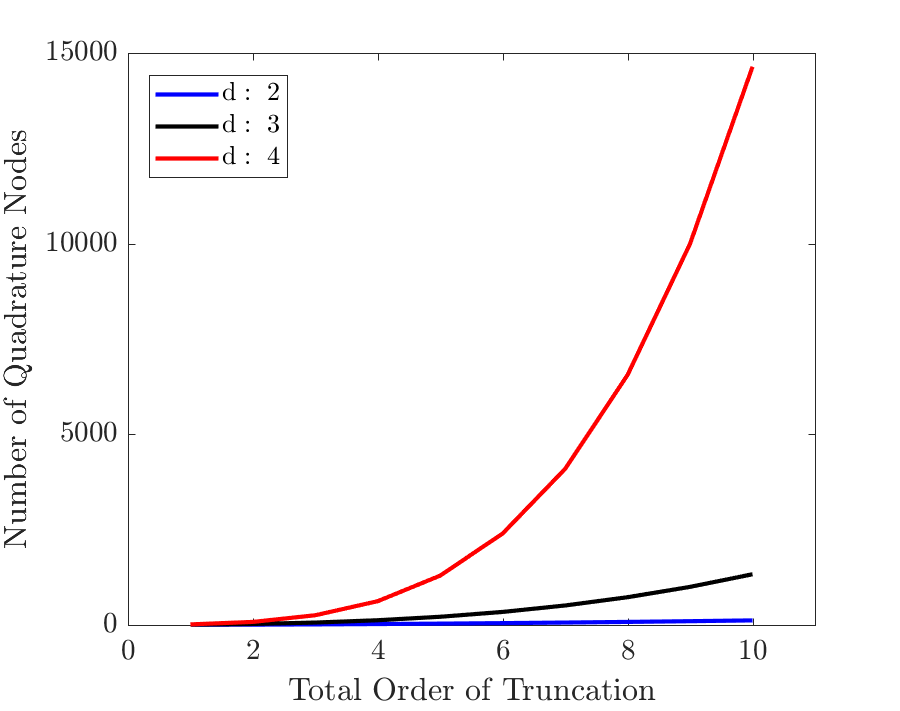
\includegraphics[width=0.7\textwidth]{./Figures/quad_comp}
\end{figure}

\end{frame}

%___________________________NEW SLIDE______________________________________

\subsection{setup}
\begin{frame}{Motivation: DGSM}

\begin{itemize}
\myitem Sensitivity analysis based on Sobol indices is commonly used to determine
relative importance of the parameters. 
\vspace{2mm}
\myitem Sobol sensitivity indices are compute intensive:
\begin{equation}
 \mathcal{T}(\theta_i) = \frac{\mathbb{E}_{\bm{\theta}\sim i}[\mathbb{V}_{\theta_i}(\mathcal{G}|\bm{\theta}_{\sim i})]}{\mathbb{V}(\mathcal{G})} \nonumber
\end{equation}
\vspace{2mm}
\myitem Bounds on Sobol indices can be computed easily using DGSM and are shown to converge at a 
much faster rate. 

\end{itemize}

\end{frame}
%___________________________NEW SLIDE______________________________________

\section{\scshape DGSM}
\subsection{dgsm}
\begin{frame}{DGSM}

\begin{itemize}
\myitem DGSM for Randomly distributed parameters 
\footnotesize{[Sobol and Kucherenko, 2009]}:\vspace{2mm}

\normalsize
\be
\mu_i = \mathbb{E}\left[\left(\frac{\partial G(\bm{x})}{\partial x_i}\right)^{2}\right]
\nonumber
\ee

where,

\be
\frac{\partial G(\bm{x}^{\ast})}{\partial x_i} = \lim_{\delta\to 0}
\frac{[G(x_1^{*},\ldots,x_{i-1}^{*},x_i^{*}+\delta,x_{i+1}^{*},\ldots,x_d^{*}) - G(\bm{x}^{*})]}{\delta} \nonumber
\ee

\myitem Total number of model realizations required to compute $\mu_i$ using $N$ samples
is $N(d+1)$.

\end{itemize}

\end{frame}

%___________________________NEW SLIDE______________________________________

\subsection{dgsm}
\begin{frame}{Bounds on Sobol Indices}

\begin{itemize}

\myitem Upper bound ($UB_i$) on Sobol Total Effect index 
($ST_i$)~\footnotesize{[Sobol and Kucherenko, 2009]}:

\normalsize
\be
ST_i \leq \frac{\mathcal{C}_i\mu_i}{V}~(\propto \hat{\mathcal{C}_i\mu_i}) \nonumber
\ee

\be
\hat{\mathcal{C}_i\mu_i} = \frac{\mathcal{C}_i\mu_i}{\sum_i \mathcal{C}_i\mu_i} \nonumber
\ee
\begin{center}
\tiny {$\mathcal{C}$: Poincar\'e Constant\hspace{3mm}  $V$: Variance}
\end{center}

\normalsize
\vspace{2mm}
\myitem The Poincar\'e Constant is specific to a given probability distribution:

\vspace{1mm}
\begin{center}
{\renewcommand{\arraystretch}{1.5}
\begin{tabular}{|p{1.5cm}|p{1.5cm}|}
 \hline
\footnotesize $\mathcal{U}[a,b]$ & \footnotesize $(b-a)^{2}/\pi^2$ \\ \hline
\footnotesize $\mathcal{N}(\mu,\sigma^2)$ & \footnotesize $\sigma^2$ \\ \hline
\end{tabular}
}
\end{center}

\end{itemize}
\end{frame}
%
%%___________________________NEW SLIDE______________________________________
%
\section{\scshape Morris}
\subsection{tc1}
\begin{frame}{Reduced Morris Function}

\vspace{-3mm}
\begin{center}
\be
f(x) = \sum_{i=1}^{4}b_ix_i + \sum_{i\leq j}^{4} b_{ij}x_ix_j + \sum_{i\leq j\leq k=4}^{4} b_{ijk}x_ix_jx_k \nonumber
\ee

$x_i\sim\mathcal{U}[0,1]$ \\

\scriptsize{
\[
b_i = 
\begin{bmatrix}
0.05 \\ 0.59 \\ 10 \\ 0.21
\end{bmatrix},~
b_{ij} = 
\begin{bmatrix}
0 & 80 &60 &40 \\ 0 & 30 & 0.73 & 0.18 \\ 0 & 0 & 0.64 &0.93 \\ 0 & 0 & 0 & 0.06
\end{bmatrix},~
b_{ij4} = 
\begin{bmatrix}
0 & 10 & 0.98 & 0.19 \\ 0 & 0 & 0.49 & 50 \\ 0 & 0 & 0 & 1 \\ 0 & 0 & 0 & 0
\end{bmatrix}
\]

}
\end{center}

\end{frame}
%
%%___________________________NEW SLIDE______________________________________
%
\subsection{tc1}
\begin{frame}{Parameter Screening}
\begin{center}
\begin{tikzpicture}
\hspace{-5mm}
\tiny
{\onslide<1->
\node (case_f) [outer]{$ST_i$: 10$^5$ Samples};
\node (x1_f) [x1,below of=case_f,yshift=0.2cm] {$x_1$: 0.4323};
\node (x2_f) [x2, below of=x1_f,yshift=0.2cm] {$x_2$: 0.4051};
\node (x4_f) [x4, below of=x2_f,yshift=0.2cm] {$x_4$: 0.1300};
\node (x3_f) [x3, below of=x4_f,yshift=0.2cm] {$x_3$: 0.0928};
}

{\onslide<3->
\node (case_10) [outer,left of=case_f,xshift=-1.5cm]{$UB_i$: 10 Samples};
\node (x1_10) [x1,left of=x1_f,xshift=-1.5cm] {$x_1$: 0.6926};
\node (x2_10) [x2, left of=x2_f,xshift=-1.5cm] {$x_2$: 0.6804};
\node (x4_10) [x4, left of=x4_f,xshift=-1.5cm] {$x_4$: 0.2531};
\node (x3_10) [x3, left of=x3_f,xshift=-1.5cm] {$x_3$: 0.1443};
}

{\onslide<2->
\node (case_5) [outer,left of=case_10,xshift=-1.5cm]{$UB_i$: 5 Samples};
\node (x1_5) [x1,left of=x1_10,xshift=-1.5cm] {$x_1$: 1.4539};
\node (x2_5) [x2, left of=x2_10,xshift=-1.5cm] {$x_2$: 1.3303};
\node (x4_5) [x4, left of=x4_10,xshift=-1.5cm] {$x_4$: 0.3761};
\node (x3_5) [x3, left of=x3_10,xshift=-1.5cm] {$x_3$: 0.3374};
}

\end{tikzpicture}
\end{center}

\end{frame}
%
%%___________________________NEW SLIDE______________________________________
%
\subsection{tc1}
\begin{frame}{PCE Convergence}

\begin{columns}
\begin{column}{0.4\textwidth}
\scriptsize{
\be
\epsilon_{LOO} = \frac{\sum_{i=1}^{N}\left(\mathcal{M}(\bm{x}^{(i)}) - 
\mathcal{M}^{PCE\setminus i}(\bm{x}^{(i)})\right)^{2}}{\sum_{i=1}^{N}
\left(\mathcal{M}(\bm{x}^{(i)}) - \hat{\mu}_Y\right)^2} \nonumber
\ee

\be
\hat{\mu}_{Y} = \frac{1}{N}\sum_{i=1}^{N}\mathcal{M}(\bm{x}^{(i)})
\nonumber
\ee
}
\end{column}
\hspace{3mm}
\begin{column}{0.6\textwidth}

\begin{figure}[htbp]
  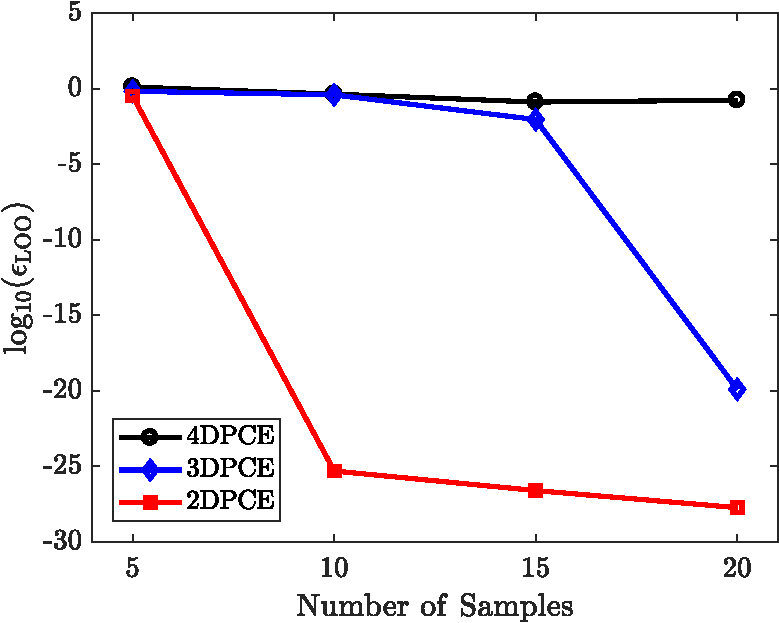
\includegraphics[width=1.0\textwidth]{./Figures/err_samples_morris}
\end{figure}

\end{column}

\end{columns}

\vspace{2mm}
\begin{itemize}
\myitem The PCE is constructed using Least Angle Regression with Latin Hypercube Sampling.
\end{itemize}

\end{frame}
%
%%___________________________NEW SLIDE______________________________________
%
\subsection{tc1}
\begin{frame}{PCE Verification}

\begin{itemize}
\myitem Generate an independent set of validation points in the 4D input parameter space.
\vspace{2mm}
\myitem Compute the following error:
\be
\epsilon_{val} = \frac{\left[\sum_{i=1}^{N}\left(\mathcal{M}(\bm{x}^{(i)}) - 
\mathcal{M}^{PCE}(\bm{x}^{(i)})\right)^{2}\right]^{\frac{1}{2}}}{\left[\sum_{i=1}^{N}
\left(\mathcal{M}(\bm{x}^{(i)})\right)^2\right]^{\frac{1}{2}}} \nonumber
\ee
\vspace{2mm}
\myitem $\epsilon_{val}$ was found to be $\mathcal{O}$(10$^{-1}$) in the case
of 4D PCE and 2D PCE constructed using {\color{blue}15} and {\color{blue}5} training 
points respectively. 
\end{itemize}

\end{frame}
%
%%___________________________NEW SLIDE______________________________________
%
\section{\scshape Borehole}
\subsection{tc2}
\begin{frame}{The Borehole Function}

\begin{columns}
\begin{column}{0.5\textwidth}
\scriptsize{
\be
\mathcal{Q} = \frac{2\pi T_u(H_u - H_l)}{\ln\left(\frac{r}{r_w}\right)\left(1 + 
\frac{2LT_u}{\ln\left(\frac{r}{r_w}\right)r_w^2K_w} + \frac{T_u}{T_l}\right)}
\nonumber
\ee
\begin{center}
\tiny $\mathcal{Q}$: Discharge of water through a borehole
\end{center}
}
\vspace{3mm}
\begin{tabular}{|p{0.15cm}|p{1.5cm}|p{3.2cm}|}
 \hline
%\textbf{Parameter} & \textbf{Distribution} & \textbf{Description} \\
\tiny $r_w$ & \tiny $\mathcal{N}$(0.1,0.016) & \tiny Radius of the borehole (m) \\
\tiny $r$ & \tiny $\log\mathcal{N}$(7.71,1.006) & \tiny Radius of influence (m) \\
\tiny $T_u$ & \tiny$\mathcal{U}$[63070,115600] & \tiny Transmissivity of upper 
aquifer (m$^2$/yr) \\
\tiny $H_u$ & \tiny$\mathcal{U}$[990,1110] & \tiny Potentiometric head of upper 
aquifer (m) \\
\tiny $T_l$ & \tiny$\mathcal{U}$[63.1,116] & \tiny Transmissivity of lower
aquifer (m$^2$/yr) \\
\tiny $H_l$ & \tiny$\mathcal{U}$[700,820] & \tiny Potentiometric head of lower 
aquifer (m) \\
\tiny $L$ & \tiny$\mathcal{U}$[1120,1680] & \tiny Length of borehole (m) \\
\tiny $K_w$ & \tiny$\mathcal{U}$[9855,12045] & \tiny Hydraulic conductivity of borehole (m/yr)\\
\hline
\end{tabular}

\end{column}
\hspace{5mm}
\begin{column}{0.5\textwidth}

\begin{figure}[htbp]
  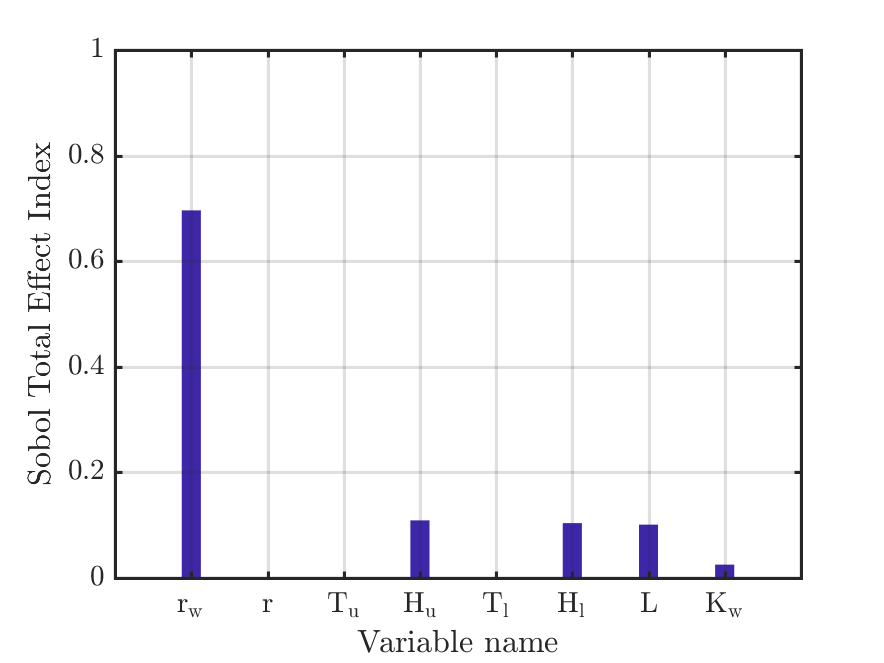
\includegraphics[width=1.1\textwidth]{./Figures/sense_bore}
\end{figure}

\end{column}

\end{columns}

\end{frame}
%%___________________________NEW SLIDE______________________________________
%
\subsection{tc2}
\begin{frame}{Parameter Screening}
\begin{center}
\begin{tikzpicture}
\hspace{-5mm}
\tiny
{\onslide<1->
\node (case_f) [outer]{$ST_i$: 10$^5$ Samples};
\node (x1_f) [x1,below of=case_f,yshift=0.2cm] {$x_1$: 0.6942};
\node (x3_f) [x3, below of=x1_f,yshift=0.2cm] {$x_3$: 0.1062};
\node (x5_f) [x5, below of=x3_f,yshift=0.2cm] {$x_5$: 0.1059};
\node (x6_f) [x6, below of=x5_f,yshift=0.2cm] {$x_6$: 0.1026};
\node (x7_f) [x7, below of=x6_f,yshift=0.2cm] {$x_7$: 0.0250};
\node (x2_f) [x2, below of=x7_f,yshift=0.2cm] {$x_2$: 0.0000};
\node (x4_f) [x4, below of=x2_f,yshift=0.2cm] {$x_4$: 0.0000};
}

{\onslide<4->
\node (case_15) [outer,left of=case_f,xshift=-1.5cm]{$UB_i$: 15 Samples};
\node (x1_15) [x1,below of=case_15,yshift=0.2cm] {$x_1$: 0.8384};
\node (x3_15) [x3, below of=x1_15,yshift=0.2cm] {$x_3$: 0.1472};
\node (x5_15) [x5, below of=x3_15,yshift=0.2cm] {$x_5$: 0.1472};
\node (x6_15) [x6, below of=x5_15,yshift=0.2cm] {$x_6$: 0.1437};
\node (x7_15) [x7, below of=x6_15,yshift=0.2cm] {$x_7$: 0.0360};
\node (x2_15) [x2, below of=x7_15,yshift=0.2cm] {$x_2$: 0.0000};
\node (x4_15) [x4, below of=x2_15,yshift=0.2cm] {$x_4$: 0.0000};
}

{\onslide<3->
\node (case_10) [outer,left of=case_15,xshift=-1.5cm]{$UB_i$: 10 Samples};
\node (x1_10) [x1,below of=case_10,yshift=0.2cm] {$x_1$: 0.8671};
\node (x3_10) [x3, below of=x1_10,yshift=0.2cm] {$x_3$: 0.1505};
\node (x5_10) [x5, below of=x3_10,yshift=0.2cm] {$x_5$: 0.1505};
\node (x6_10) [x6, below of=x5_10,yshift=0.2cm] {$x_6$: 0.1466};
\node (x7_10) [x7, below of=x6_10,yshift=0.2cm] {$x_7$: 0.0337};
\node (x2_10) [x2, below of=x7_10,yshift=0.2cm] {$x_2$: 0.0000};
\node (x4_10) [x4, below of=x2_10,yshift=0.2cm] {$x_4$: 0.0000};
}

{\onslide<2->
\node (case_5) [outer,left of=case_10,xshift=-1.5cm]{$UB_i$: 5 Samples};
\node (x1_5) [x1,below of=case_5,yshift=0.2cm] {$x_1$: 0.2124};
\node (x6_5) [x6, below of=x1_5,yshift=0.2cm] {$x_6$: 0.0406};
\node (x3_5) [x3, below of=x6_5,yshift=0.2cm] {$x_3$: 0.0393};
\node (x5_5) [x5, below of=x3_5,yshift=0.2cm] {$x_5$: 0.0393};
\node (x7_5) [x7, below of=x5_5,yshift=0.2cm] {$x_7$: 0.0089};
\node (x2_5) [x2, below of=x7_5,yshift=0.2cm] {$x_2$: 0.0000};
\node (x4_5) [x4, below of=x2_5,yshift=0.2cm] {$x_4$: 0.0000};
}

\end{tikzpicture}
\end{center}

\end{frame}
%
%%___________________________NEW SLIDE______________________________________
%
\subsection{tc1}
\begin{frame}{PCE Convergence and Verification}

\begin{figure}[htbp]
  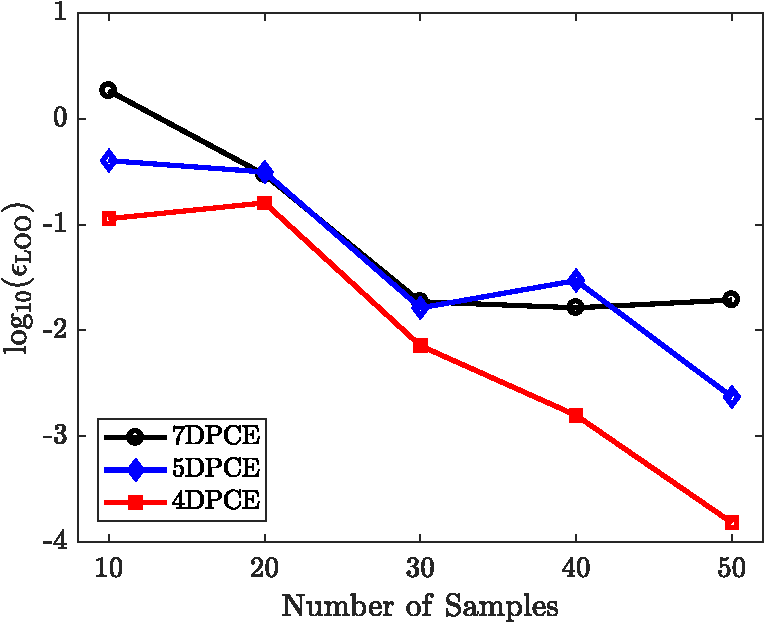
\includegraphics[width=0.65\textwidth]{./Figures/err_samples_borehole}
\end{figure}

\begin{itemize}
\myitem $\epsilon_{val}$ was found to be $\mathcal{O}$(10$^{-2}$) in the case
of 7D PCE and 4D PCE constructed using {\color{blue}60} and {\color{blue}30}
training points respectively.
\end{itemize}

\end{frame}

%%___________________________NEW SLIDE______________________________________
%
\section{\scshape Oscillator}
\subsection{osc}
\begin{frame}{Non-Linear Oscillator}

\begin{columns}
\begin{column}{0.5\textwidth}

\begin{figure}[htbp]
  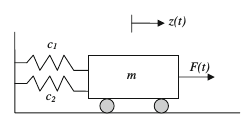
\includegraphics[width=0.95\textwidth]{./Figures/oscillator}
\end{figure}

\vspace{1mm}
\textbf{Limit State Function}:
\vspace{-1mm}

\be
g(\bm{X}) = 3r - \left|\frac{2F}{m\omega_0^2}\sin\left(\frac{\omega_0t_1}{2}\right)\right|
\nonumber
\ee

\begin{center}
\scriptsize
$\bm{X}~=~\{m,k_1,k_2,r,F,t_1\}$ \hspace{3mm} $\omega_0~=~\sqrt{\frac{c_1+c_2}{m}}$ 
\end{center}

\end{column}

\begin{column}{0.5\textwidth}

\begin{center}
\vspace{-4mm}
\begin{tabular}{|p{0.15cm}|p{1.2cm}|p{1.7cm}|}
 \hline
%\textbf{Parameter} & \textbf{Distribution} & \textbf{Description} \\
\tiny $m$ & \tiny $\mathcal{N}$(1,0.05) & \tiny Mass \\
\tiny $k_1$ & \tiny $\mathcal{N}$(1,0.1) & \tiny Spring Constant \\
\tiny $k_2$ & \tiny $\mathcal{N}$(0.1,0.01) & \tiny Spring Constant \\
\tiny $r$ & \tiny $\mathcal{N}$(0.5,0.05) & \tiny Displacement \\
\tiny $F$ & \tiny $\mathcal{N}$(1,0.2) & \tiny Force \\
\tiny $t_1$ & \tiny $\mathcal{N}$(1,0.2) & \tiny Time \\
\hline
\end{tabular}

\hspace{-2mm}
\begin{figure}[htbp]
\vspace{-2mm}
  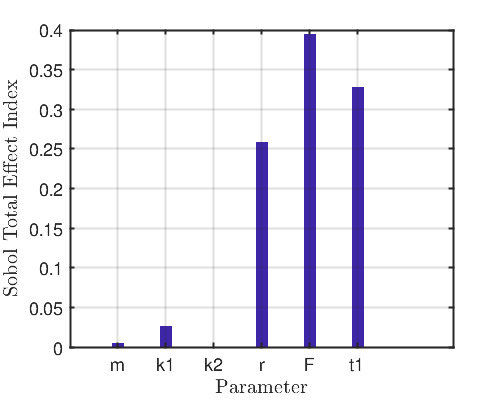
\includegraphics[width=0.95\textwidth]{./Figures/sens_oscillator}
\end{figure}

\end{center}

\end{column}
\end{columns}

\end{frame}

%%___________________________NEW SLIDE______________________________________
%
\subsection{osc}
\begin{frame}{Parameter Rank Metric}

\begin{columns}
        \begin{column}{0.5\textwidth}

\begin{center}
\be
\hat{\mathcal{C}_i\mu_i} = \frac{\mathcal{C}_i\mu_i}{\sum_i \mathcal{C}_i\mu_i} \nonumber
\ee
\tiny {$\mathcal{C}$: Poincar\'e Constant\hspace{3mm} $\mu_i$: DGSM}

\end{center}

\end{column}

\hspace{-10mm}
 \begin{column}{0.5\textwidth}
 
 \begin{figure}[htbp]
        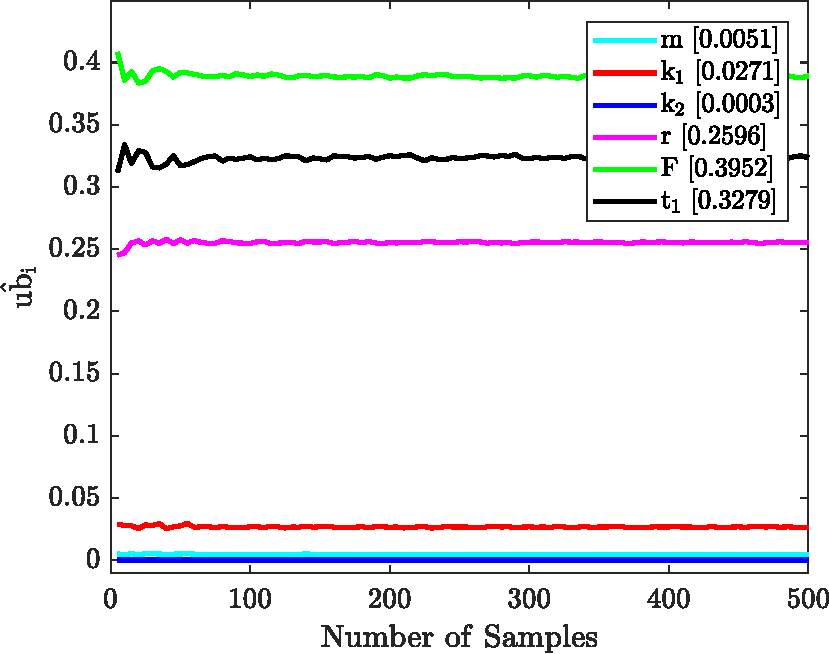
\includegraphics[width=1.1\textwidth]{./Figures/ub_conv_oscillator}
\end{figure}
 
 \end{column}
 \end{columns}
 

\end{frame}

%%___________________________NEW SLIDE______________________________________
%
\subsection{osc}
\begin{frame}{PCE Convergence}

 \begin{figure}[htbp]
        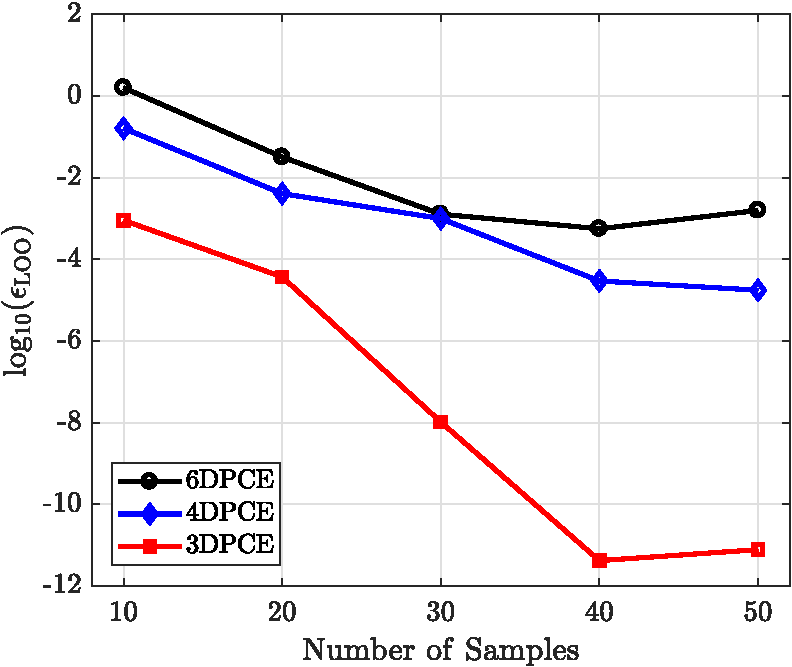
\includegraphics[width=0.65\textwidth]{./Figures/err_samples_oscillator}
\end{figure}

\end{frame}

%%___________________________NEW SLIDE______________________________________
%
\subsection{osc}
\begin{frame}{PCE Verification}

\begin{itemize}
\myitem Relative L-2 norm of the error is computed:

\tiny
\be
\epsilon_{val} = \frac{\left[\sum_{i=1}^{N}\left(\mathcal{M}(\bm{x}^{(i)}) - 
\mathcal{M}^{PCE}(\bm{x}^{(i)})\right)^{2}\right]^{\frac{1}{2}}}{\left[\sum_{i=1}^{N}
\left(\mathcal{M}(\bm{x}^{(i)})\right)^2\right]^{\frac{1}{2}}} = 8.35\times10^{-2}
\nonumber
\ee

\normalsize
\vspace{2mm}
\myitem Comparison of PDFs:

 \begin{figure}[htbp]
        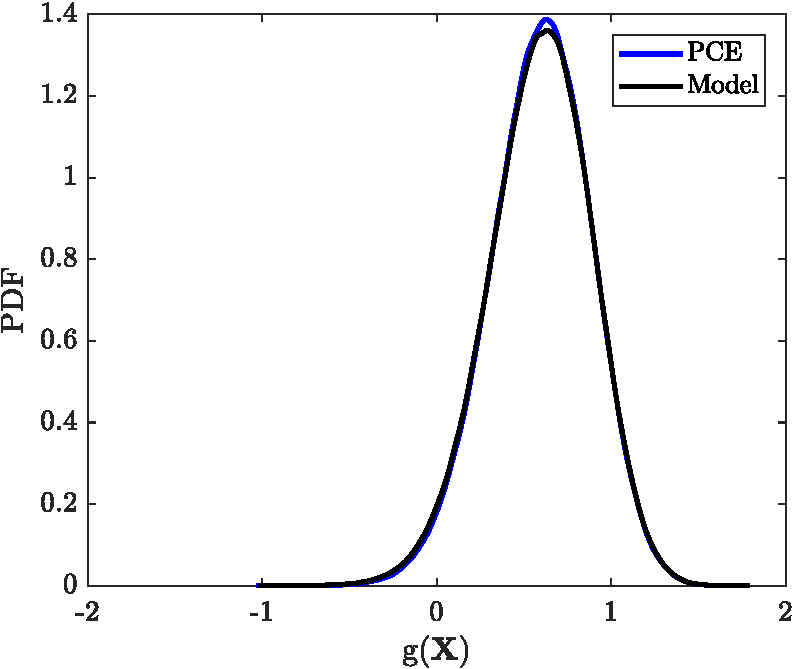
\includegraphics[width=0.45\textwidth]{./Figures/pdf_comp_oscillator}
\end{figure}

 
\end{itemize}


\end{frame}

%%___________________________NEW SLIDE______________________________________
%
\section{\scshape Elliptic PDE}
\subsection{elliptic}
\begin{frame}{Elliptic PDE}

\begin{columns}

\begin{column}{0.5\textwidth}


\be
-\kappa \Delta u + cu^3 = q \nonumber
\ee
\tiny
\be
q = (-2\pi^2)(a\cos(2\pi x)\sin^2(\pi y) + b\cos(2\pi y)\sin^2(\pi x)) \nonumber
\ee

\begin{center}

{\renewcommand{\arraystretch}{1.5}
\begin{tabular}{|p{0.15cm}|p{1.8cm}|}
 \hline
\scriptsize {$\kappa$} & \scriptsize {$\mathcal{U}$[0.09, 0.11]} \\
\scriptsize {$c$} & \scriptsize {$\mathcal{U}$[0.9, 1.1]} \\
\scriptsize {$a$} & \scriptsize {$\mathcal{U}$[0.9, 1.1]} \\
\scriptsize {$b$} & \scriptsize {$\mathcal{U}$[0.9, 1.1]} \\
\hline
\end{tabular}
}
\end{center}

\end{column}

\begin{column}{0.5\textwidth}
\vspace{-7mm}
 \begin{figure}[htbp]
        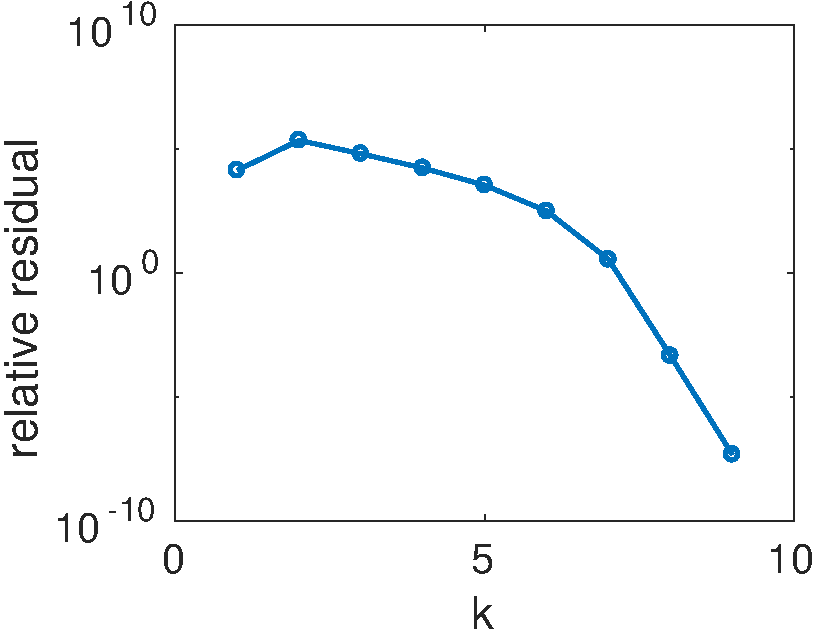
\includegraphics[width=1.0\textwidth]{./Figures/u_soln}
\end{figure}

\vspace{-9mm}

\begin{figure}[htbp]
        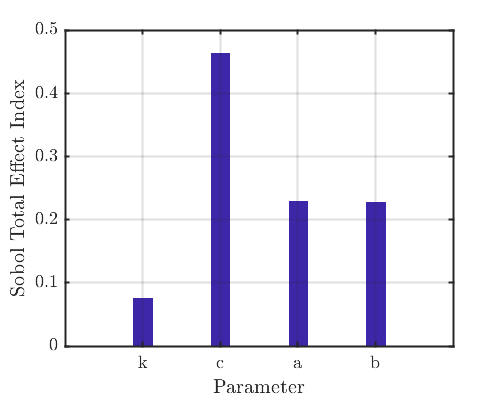
\includegraphics[width=0.85\textwidth]{./Figures/sens_elliptic}
\end{figure}

\end{column}
\end{columns}

\end{frame}

%%___________________________NEW SLIDE______________________________________
%
\subsection{elliptic}
\begin{frame}{Analysis}

\vspace{-2mm}
\begin{columns}

\begin{column}{0.5\textwidth}

\begin{center}
\tiny{Parameter Screening}
\vspace{-2mm}
 \begin{figure}[htbp]
   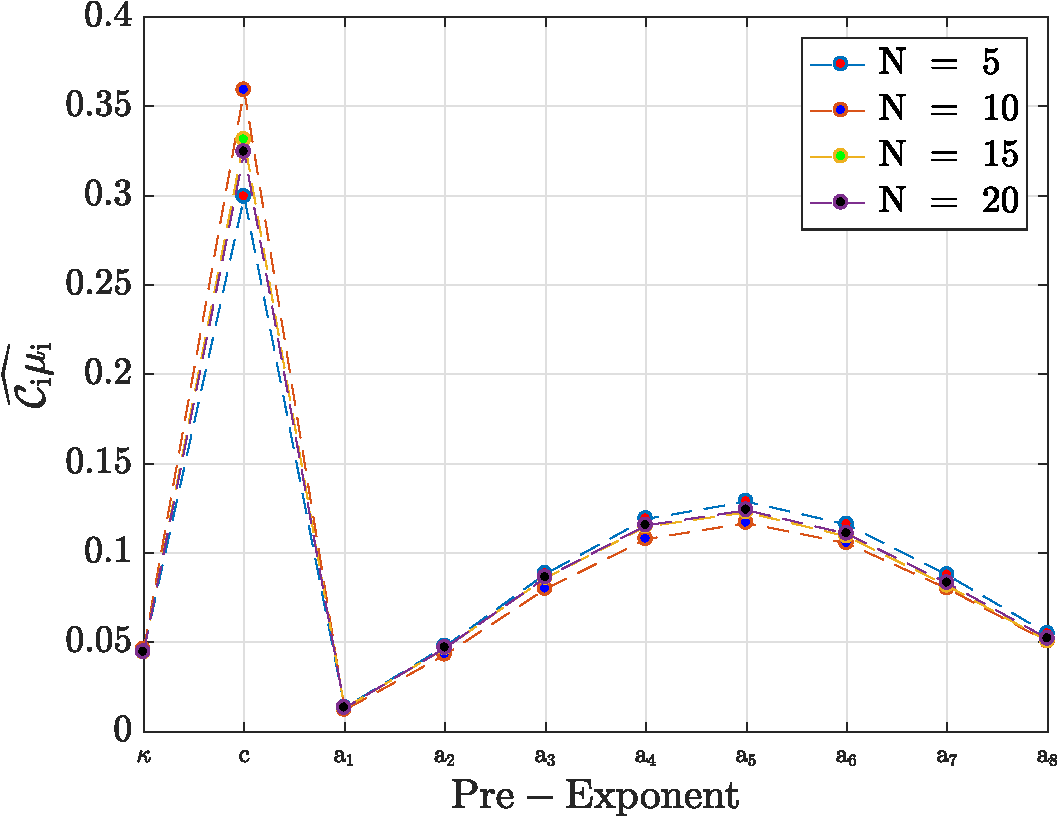
\includegraphics[width=0.75\textwidth]{./Figures/ub_conv_elliptic}
\end{figure}
\end{center}

\end{column}

\begin{column}{0.5\textwidth}

\begin{center}
\tiny{Convergence}
\vspace{-2mm}
 \begin{figure}[htbp]
   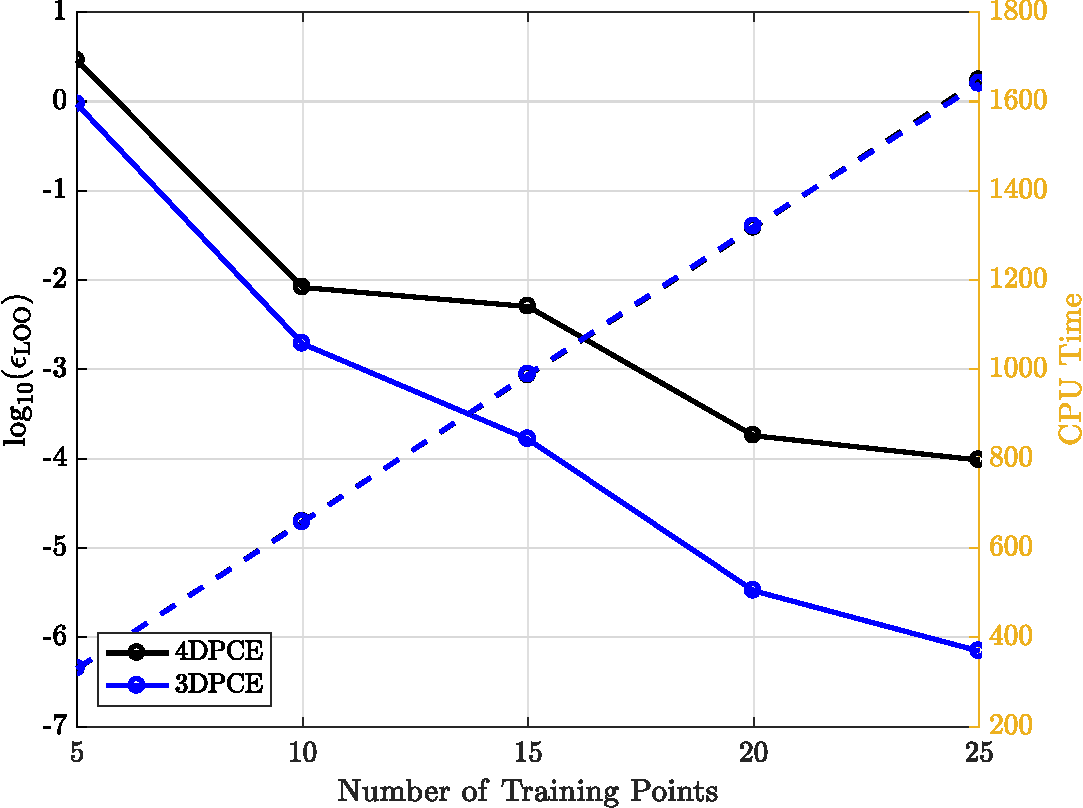
\includegraphics[width=0.75\textwidth]{./Figures/err_samples_elliptic}
\end{figure}
\end{center}

\end{column}

\end{columns}

\begin{center}
\tiny{Verification}
\vspace{-2mm}
 \begin{figure}[htbp]
   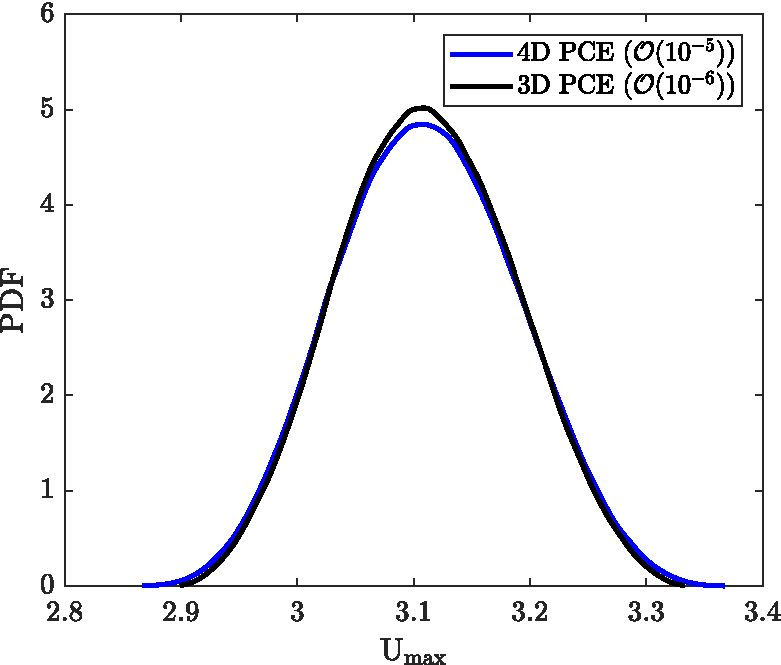
\includegraphics[width=0.35\textwidth]{./Figures/pdf_comp4Dv3D_elliptic}
\end{figure}
\end{center}

\end{frame}
%
%%___________________________NEW SLIDE______________________________________
%
\section{\scshape Algorithm}
\subsection{alg}
\begin{frame}{Algorithm: Parameter Screening}
%\textsc{Algorithm}
%\vspace{10mm}
\begin{algorithm}[H]
\SetAlgoLined
%\nonl \scriptsize{\textsc{Part I: Parameter Screening}}
\scriptsize
%\nonl \textbf{\texttt{Part I: Parameter Screening}}\;
\texttt{Generate $n_1$ points in $\mathbb{R}^{d}$}\;
\texttt{Compute $UB_i$ for parameters $\theta_i$ 
using $n_1$ points}\;
\nonl\scriptsize\texttt{\color{blue}$\%~NF$ = $n_1(d+1)$,~$NF$:~Number of
model realizations}\;
%\normalsize
\texttt{Rank Parameters $(\theta_i)$ based on $UB_i$ estimates 
($\mathcal{R}^{\tiny {old}}$)}\;
\texttt{set $k$ = 1}
\scriptsize\texttt{\color{blue}$\%$~$k$:~Iteration counter}\;
%\normalsize
\Repeat{\texttt{$\mathcal{R}^{\tiny{new}}$ $\neq$ $\mathcal{R}^{\tiny{old}}$}}{
\texttt{Generate $\beta n_1$ new points in $\mathbb{R}^{d}$ ($\beta n_1\in\mathbb{Z}$)}\;
\texttt{Compute $UB_i^{\tiny{new}}$ using (1+$\beta k)n_1$ points}\;
\nonl\scriptsize\texttt{\color{blue}$\%~NF$ = $(1+\beta k)n_1(d+1)$}\;
%\normalsize
\texttt{Rank Parameters based on $UB_i^{\tiny{new}}$ estimates
($\mathcal{R}^{\tiny{new}}$)}\;
\If {(\texttt{$\mathcal{R}^{\tiny{new}}$ = $\mathcal{R}^{\tiny{old}}$})}{
\texttt{Compute: $r_i$ = $\frac{UB_i^{\tiny{new}}}{max(UB_i^{\tiny{new}})}$}\;
\texttt{Construct a set $s$ = $\{\theta_i~\ni~r_i<\alpha\}$}\;
\texttt{Exit the loop}\;
}
\texttt{set $k$ = $k$ + 1}\;
}
\texttt{Construct a validation set: ($\bm{\theta}_j$,$\mathcal{M}(\bm{\theta}_j)$),
$j$=1,2,$\ldots$,$NF$}\;
\end{algorithm}
\end{frame}

%%___________________________NEW SLIDE______________________________________
%
\section{\scshape MD}
\subsection{md}
\begin{frame}{Application: Non-Equilibrium MD}

\begin{columns}
        \begin{column}{0.5\textwidth}

\begin{center}
\begin{tikzpicture}
\node[fill=white,inner sep=0pt]
{\rowcolors{1}{DeepSkyBlue!20}{DeepSkyBlue!5}
        \resizebox{\columnwidth}{!}{
  \begin{tabular}{|l|c|}\hline
          Lattice Constant ($\angstrom$) & 5.43 \\
          $W$, $H$ ($\angstrom$) & 117.94, 117.94 \\
          Temperature (K) & 300 \\
          $\Delta t$ (ps) & 0.0005 \\
          BC & Periodic \\
          Structure & Diamond \\
          Potential, $\Phi$ & Stillinger-Weber \\
  \hline
  \end{tabular}%
        }
};
\end{tikzpicture}
\end{center}

\be
\Phi = f(A,B,p,q,a,\lambda,\gamma) \nonumber
\ee


\end{column}

\begin{column}{0.5\textwidth}

\begin{center}
%        \animategraphics[autoplay,poster=first,loop,height=0.60\textwidth]{5}
%        {./animation/snap}{0}{64}
\begin{figure}[htbp]
        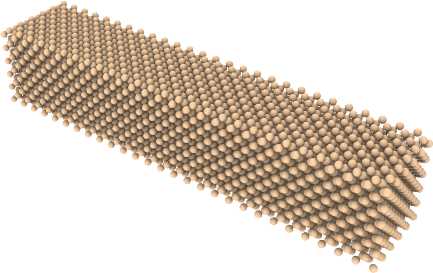
\includegraphics[width=0.9\textwidth]{./Figures/snap0}
\end{figure}
\end{center}

\vspace{-5mm}


\begin{figure}[htbp]
        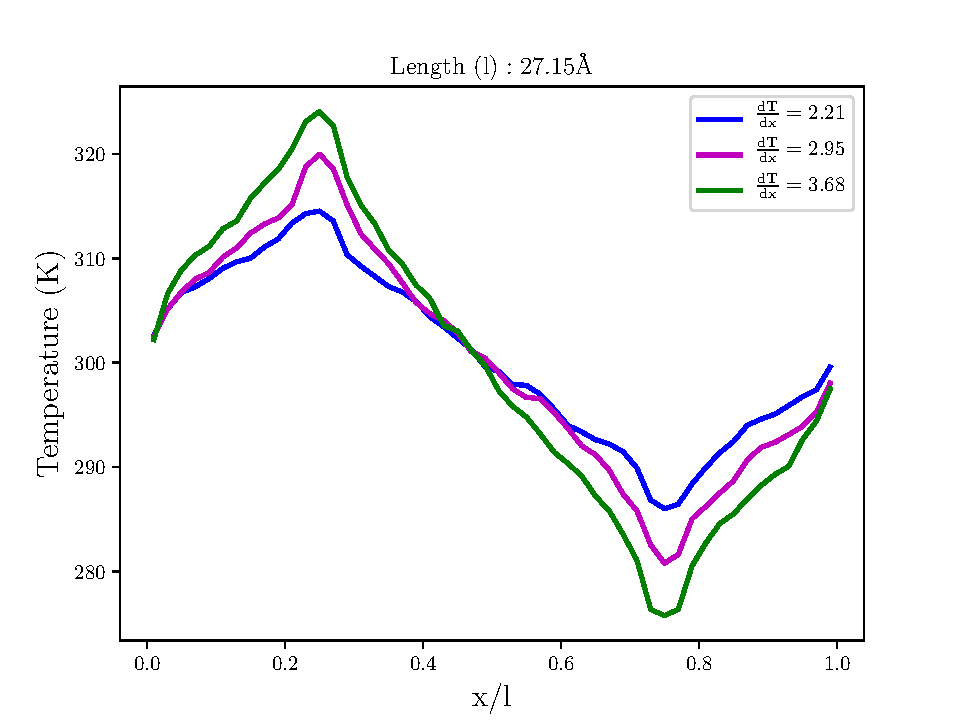
\includegraphics[width=0.9\textwidth]{./Figures/temp_plot}
\end{figure}

\end{column}

\end{columns}

\end{frame}


\end{document}


%___________________________NEW SLIDE______________________________________

%\section{\scshape Algorithm}
%\subsection{alg}
%\begin{frame}[allowframebreaks]
%
%\textsc{Algorithm}
%
%\begin{algorithmic}[1]
%\STATEx Part I: Parameter Screening
%
%\STATE \texttt{Generate an initial set of $n$ Sobol samples.} \COMMENT {\small {\color{blue}\texttt{Sobol samples explore the input parameter space uniformly and could be re-used for higher order PCEs.}}}
%
%\STATE \normalsize \texttt{Compute DGSM indices using these $n$ samples.} 
%\COMMENT{\small{\color{blue}\texttt{$\mathcal{O}(n(d+1))$: $d$ - dimensions}}}
%
%\STATE \texttt{Construct a sparse basis PCE using the $n$ samples.}
%
%\STATE \texttt{Rank Parameters based on estimates of DGSM indices or bounds on Sobol indices.}
%
%\STATE \texttt{Rank parameters using Sobol Sensitivity indices from the PCE constructed in Step 3.}
%
%\STATE \texttt{From both sets of ranks, construct a pool of parameters with $\frac{\mathcal{S}_i}{\mathcal{S}_{i,max}}$ $<$
% $\alpha$. \COMMENT {{\color{blue}Rank from Step 4 may or may not be consistent with Step 5. $\mathcal{S}_i$:
% Main effect index, $\mathcal{S}_{i,max}$: Max value of $\mathcal{S}_i$}}}
% 
% \STATE \texttt{Fix those parameters in the pool that are obtained from both approaches.}
% 
% \STATE \texttt{Construct a new PCE in the reduced input parameter space.}
% 
% \STATE \texttt{Analyze the accuracy of the newly constructed PCE in Step 8.}
% 
% \STATE \texttt{If the accuracy criterion is satisfied then terminate else add a new set of samples and repeat Steps 2--9.}
%\end{algorithmic}
%%\caption{Adaptive DGSM for PC Surrogates}
%%\label{alg:seq}
%
%\end{frame}
